% !TEX root = ../../main.tex

\subsection{BER-SE Trade-Off Across Configurations}

The previous sections examined representative OTFS-IM configurations in detail. This section combines the available simulation results into a configuration-level comparison. The purpose is not only to identify the lowest BER curve, but also to interpret each result together with its spectral efficiency. This distinction is important because an OTFS-IM configuration may improve BER by reducing the number of transmitted information bits per block, while another configuration may preserve the same spectral efficiency as the baseline OTFS system.

Two summary figures are used for this comparison. The first figure compares the BER values of different OTFS-IM configurations at selected SNR points. This view is useful for quickly identifying which configurations operate below the OTFS reference curve. The second figure places the same BER values against spectral efficiency. This view clarifies whether a BER improvement is obtained at equal spectral efficiency or by accepting a lower-rate transmission mode.

\IfFileExists{Images/Chapter5/configuration_ber_summary.png}{%
\begin{figure}[H]
    \centering
    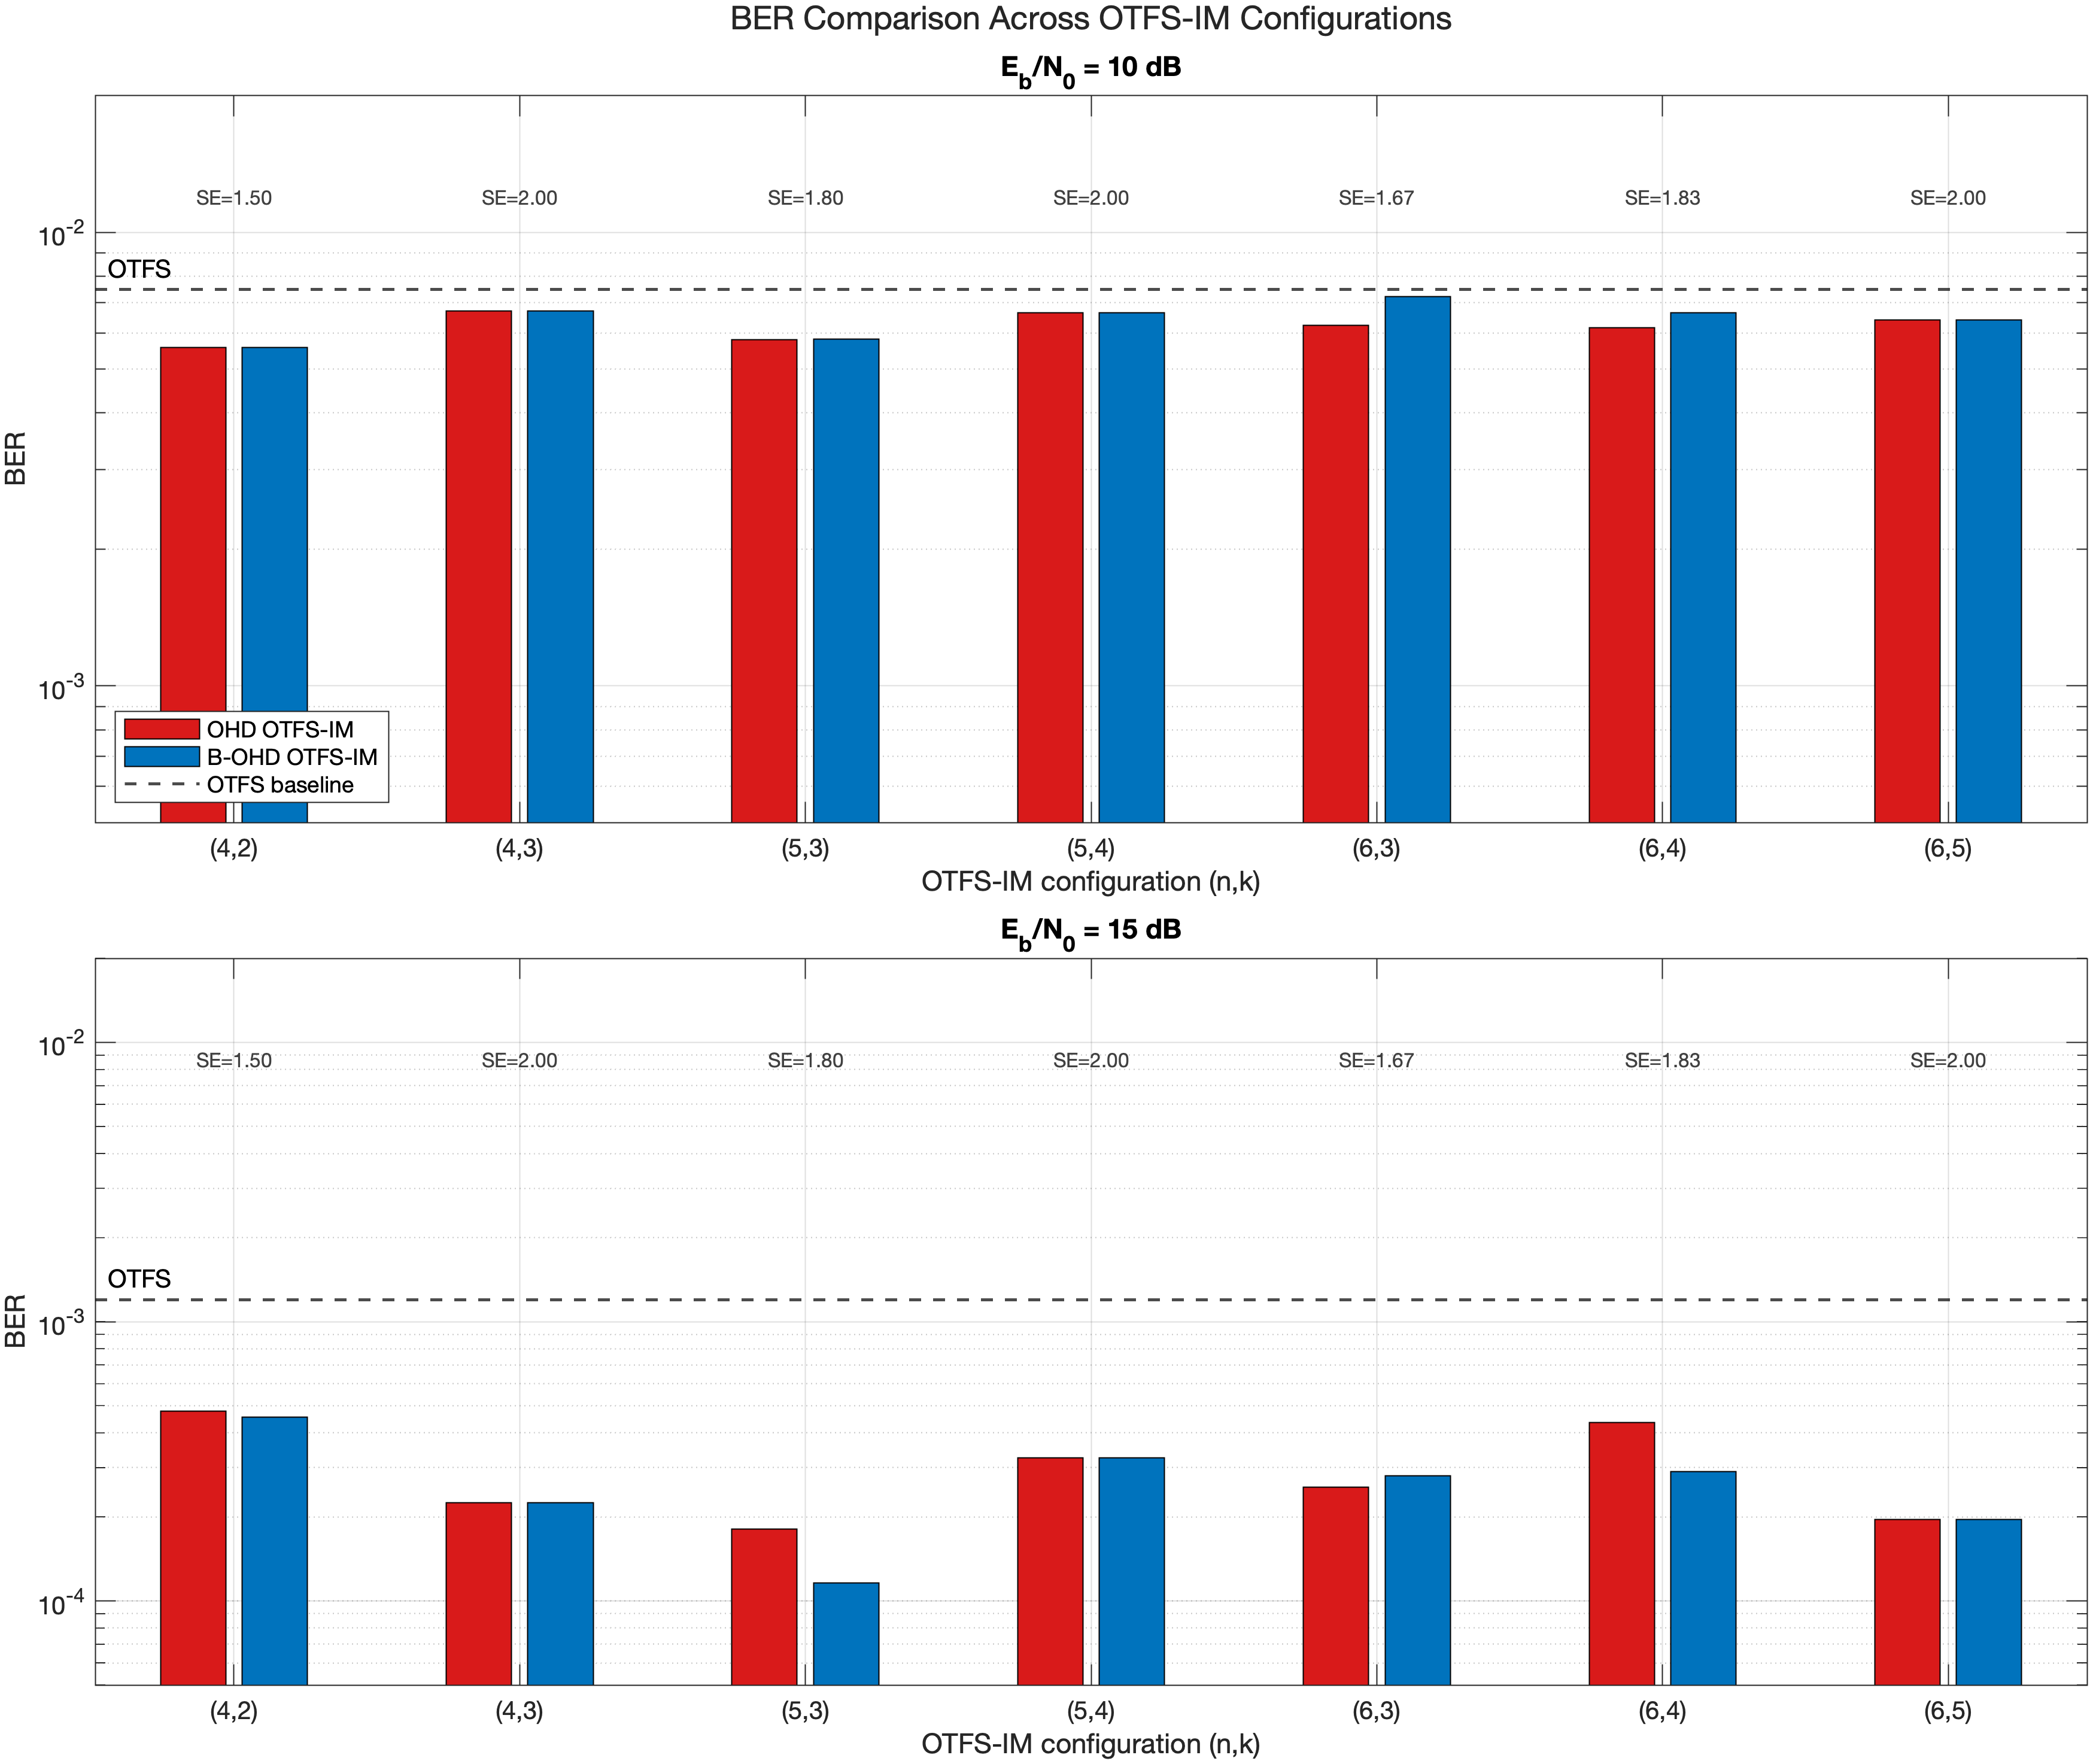
\includegraphics[width=0.95\linewidth]{Images/Chapter5/configuration_ber_summary.png}
    \caption{Configuration-level BER comparison for OHD and B-OHD OTFS-IM at selected SNR points}
    \label{fig:chapter5_configuration_ber_summary}
\end{figure}
}{%
\begin{figure}[H]
    \centering
    \fbox{%
        \begin{minipage}[c][0.28\textheight][c]{0.88\linewidth}
            \centering
            Required figure file is missing:\\
            Images/Chapter5/configuration\_ber\_summary.png
        \end{minipage}
    }
    \caption{Configuration-level BER comparison for OHD and B-OHD OTFS-IM at selected SNR points}
    \label{fig:chapter5_configuration_ber_summary}
\end{figure}
}

Figure~\ref{fig:chapter5_configuration_ber_summary} summarizes the BER of the simulated OTFS-IM configurations at \(E_b/N_0=10~\mathrm{dB}\) and \(E_b/N_0=15~\mathrm{dB}\). The dashed horizontal line represents the baseline OTFS BER at the same SNR value. Therefore, a bar below this line indicates that the corresponding OTFS-IM configuration achieves a lower BER than baseline OTFS at that operating point.

At \(10~\mathrm{dB}\), most OTFS-IM configurations are already below the OTFS baseline. However, the separation is moderate because the detector still operates in a region where both index errors and symbol errors contribute to the total BER. In this region, changing the pattern table from OHD to B-OHD does not always create a large visible gain. This behavior is consistent with the error-decomposition results: when the received reliability is still limited, the total BER is dominated not only by the geometric distance between activation patterns, but also by the quality of the MP detector output.

At \(15~\mathrm{dB}\), the difference between configurations becomes clearer. Several OTFS-IM configurations move further below the OTFS baseline, showing that index modulation can be beneficial in the medium-to-high-SNR region. The \(n=5,k=3\) case is particularly useful for pattern-selection validation because B-OHD improves over OHD while keeping the same IM block size and modulation order. This confirms that the balancing term in B-OHD can be meaningful when the selected pattern table is not identical to the OHD table. By contrast, in configurations such as \(n=6,k=5\), OHD and B-OHD may select effectively the same pattern table, so their BER curves overlap.

\IfFileExists{Images/Chapter5/ber_se_tradeoff.png}{%
\begin{figure}[H]
    \centering
    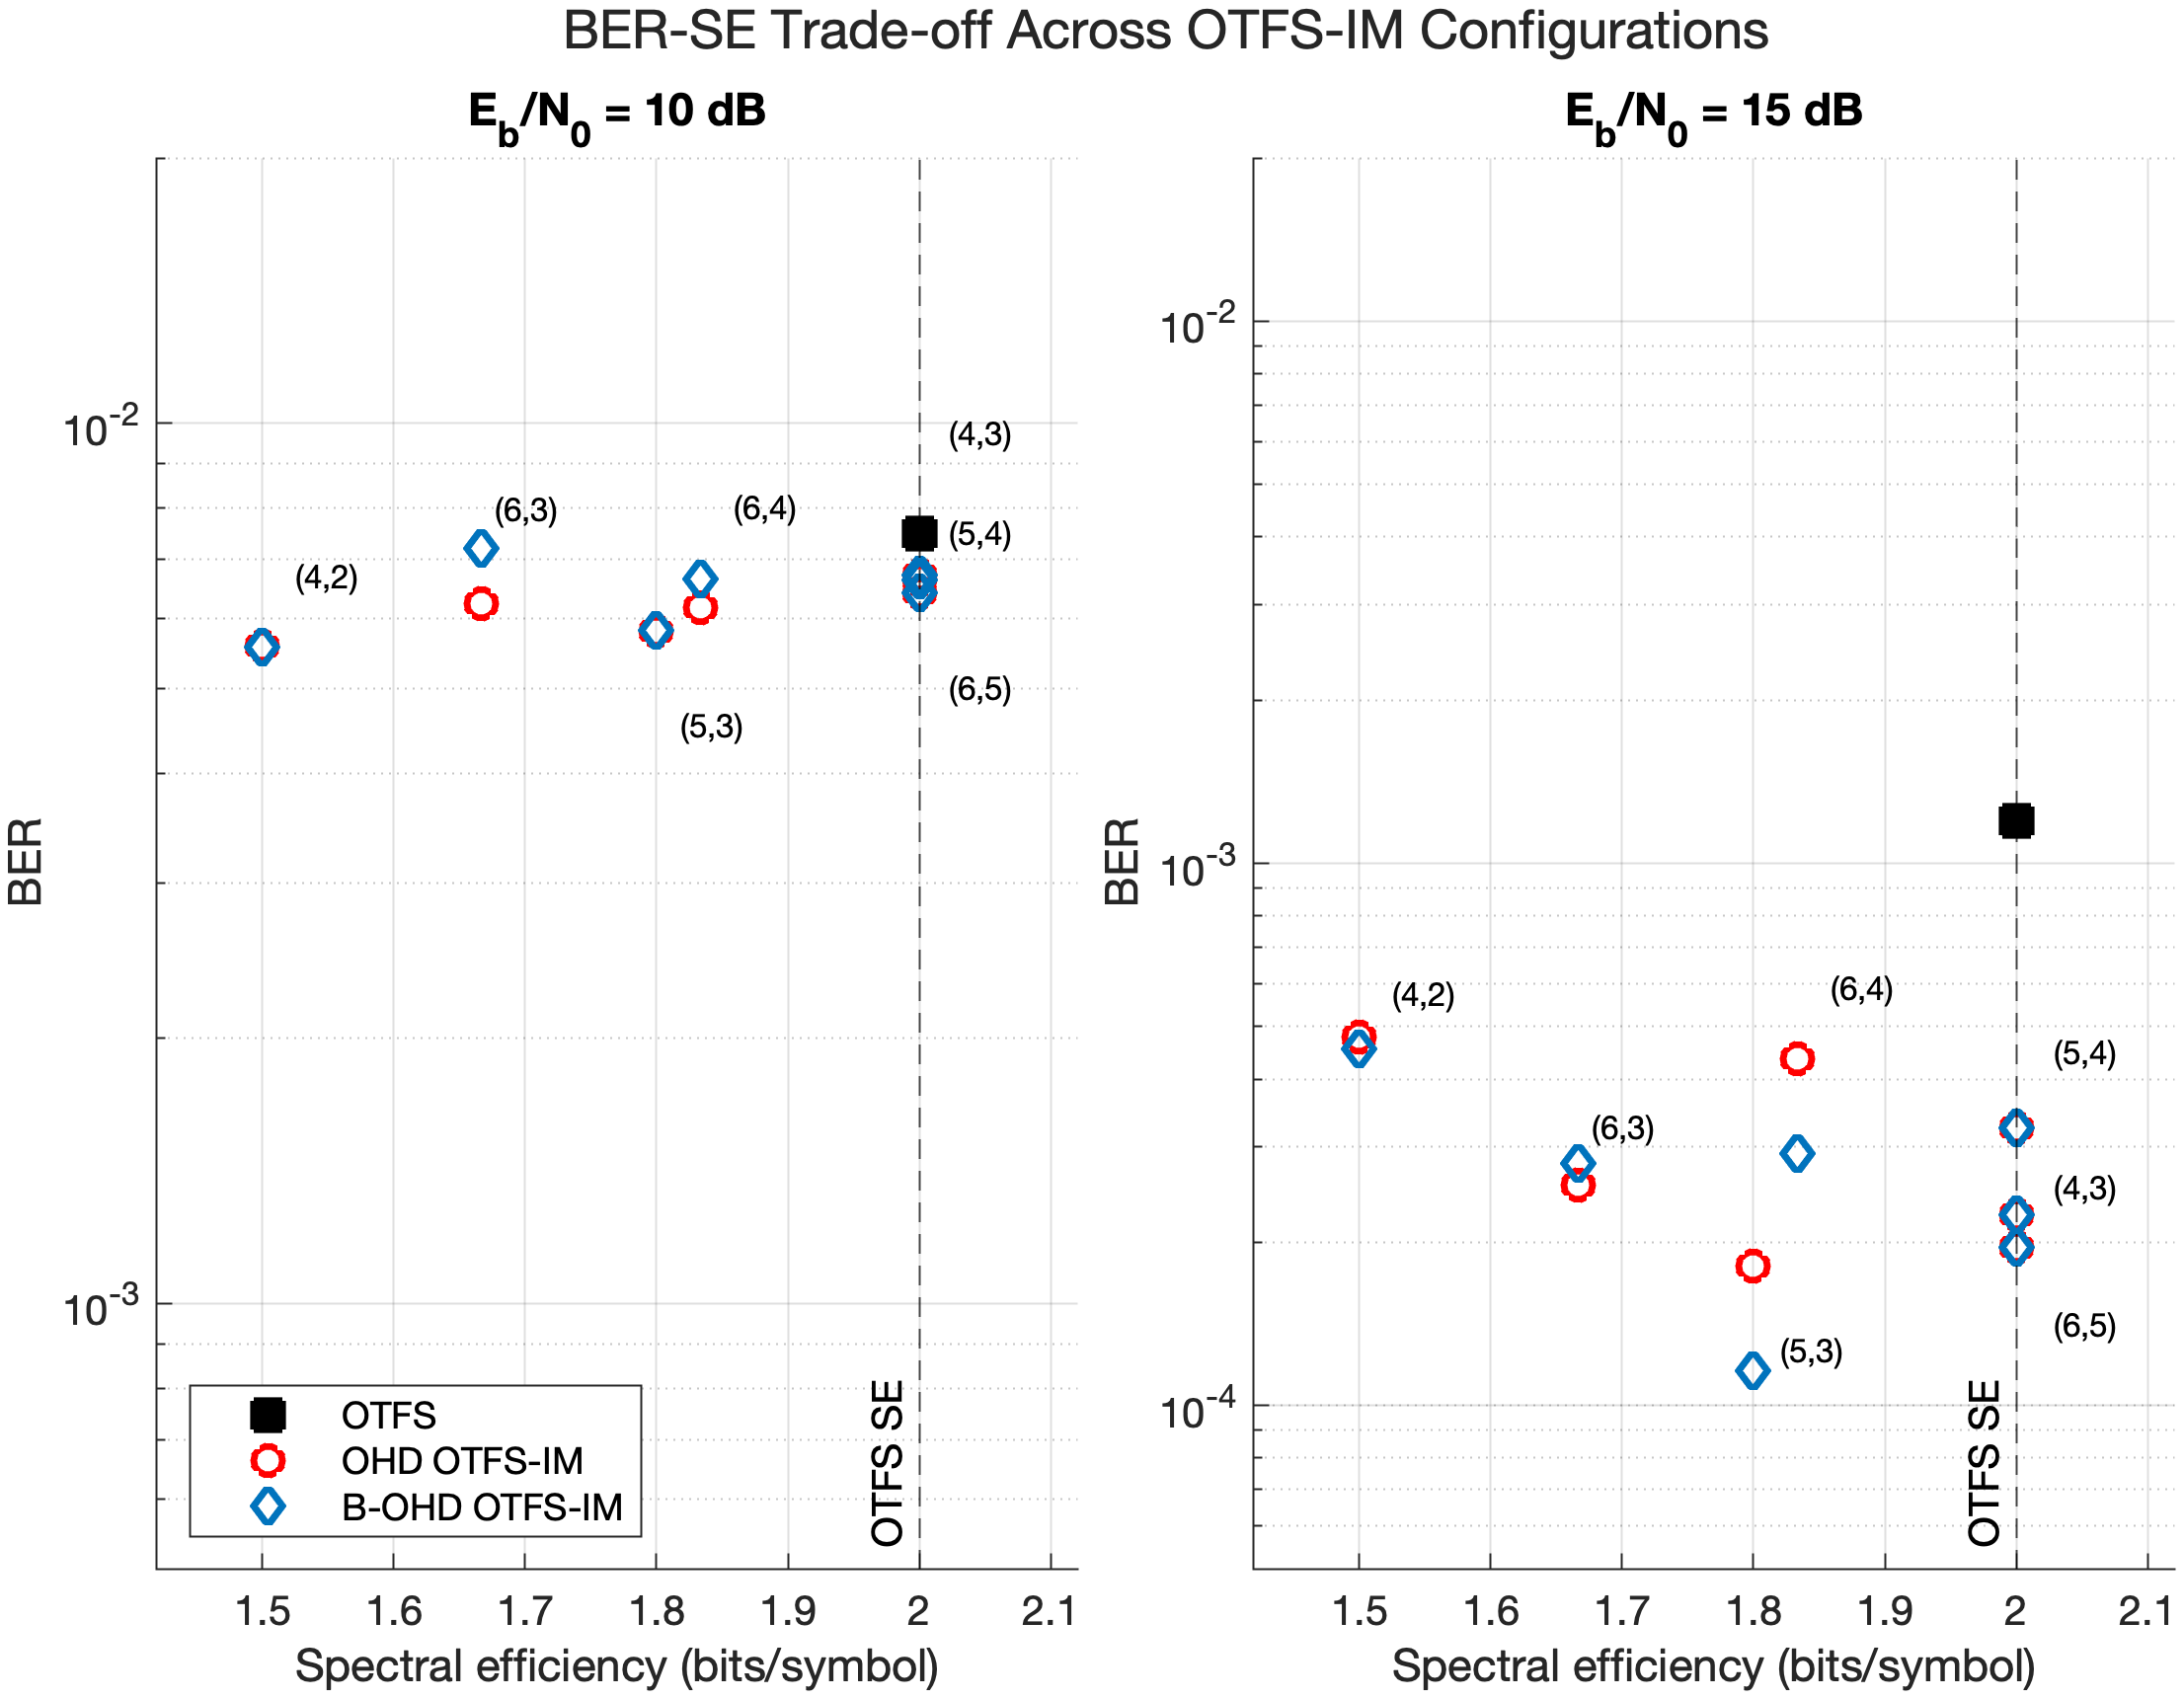
\includegraphics[width=0.95\linewidth]{Images/Chapter5/ber_se_tradeoff.png}
    \caption{BER-SE trade-off across OTFS-IM configurations at selected SNR points}
    \label{fig:chapter5_ber_se_tradeoff}
\end{figure}
}{%
\begin{figure}[H]
    \centering
    \fbox{%
        \begin{minipage}[c][0.28\textheight][c]{0.88\linewidth}
            \centering
            Required figure file is missing:\\
            Images/Chapter5/ber\_se\_tradeoff.png
        \end{minipage}
    }
    \caption{BER-SE trade-off across OTFS-IM configurations at selected SNR points}
    \label{fig:chapter5_ber_se_tradeoff}
\end{figure}
}

Figure~\ref{fig:chapter5_ber_se_tradeoff} gives a more complete interpretation of the same results. The vertical dashed line marks the spectral efficiency of the baseline OTFS system, which is \(2.00~\text{bits/symbol}\) for 4-QAM. Points located on this line correspond to equal-SE OTFS-IM configurations, while points to the left correspond to lower-SE configurations. This representation is important because a lower BER at a smaller spectral efficiency should not be interpreted in the same way as a lower BER at equal spectral efficiency.

The equal-SE configurations, including \(n=4,k=3\), \(n=5,k=4\), and \(n=6,k=5\), are the most direct comparison against baseline OTFS. These cases show that OTFS-IM can preserve the same nominal spectral efficiency while improving BER in the simulated delay-Doppler channel. Among them, the \(n=6,k=5\) configuration is the main equal-SE example used in this chapter because it has a larger IM block and provides clearer high-SNR performance separation from baseline OTFS. However, the overlap between OHD and B-OHD in this case also shows that the proposed balancing criterion does not always change the selected pattern table.

The lower-SE configurations, such as \(n=4,k=2\), \(n=5,k=3\), \(n=6,k=3\), and \(n=6,k=4\), occupy the left side of the trade-off plot. Their BER values are generally competitive because they transmit fewer information bits per block. These configurations are useful when reliability is prioritized over throughput, but their gains must be described as BER-SE trade-offs rather than pure improvements over baseline OTFS. In particular, the \(n=5,k=3\) case is valuable because it demonstrates the difference between OHD and B-OHD in a setting where exact pattern selection remains feasible and the pattern table is not trivially identical.

The comparison also shows that B-OHD should be interpreted as a refinement of OHD rather than a universally dominant detector or modulation method. B-OHD does not change the OTFS-IM signal model, the MP detector, or the modulation order. It only changes the selected activation-pattern table by adding a carrier-usage balancing criterion. Therefore, its gain appears mainly when the selected table has room for improvement in usage balance and when the detector output is reliable enough for such pattern-level differences to affect the final decision.

Overall, the BER-SE summary supports three design insights. First, OTFS-IM can outperform baseline OTFS in the simulated high-Doppler delay-Doppler channel, especially from the medium-SNR region onward. Second, equal-SE configurations are the strongest evidence that OTFS-IM is not merely improving BER by lowering the information rate. Third, pattern selection remains configuration-dependent: B-OHD can improve OHD when the OHD table is unbalanced, but random or structurally similar tables can sometimes perform competitively. For this reason, the final evaluation should report both the absolute BER curves and the BER-SE trade-off, rather than relying on a single BER plot.
